%%%%%%%%%%%%%%%%%%%%%%%%%%%%%%%%%%%%%%%%%
% FRI Data Science_report LaTeX Template
% Version 1.0 (28/1/2020)
% 
% Jure Demšar (jure.demsar@fri.uni-lj.si)
%
% Based on MicromouseSymp article template by:
% Mathias Legrand (legrand.mathias@gmail.com) 
% With extensive modifications by:
% Antonio Valente (antonio.luis.valente@gmail.com)
%
% License:
% CC BY-NC-SA 3.0 (http://creativecommons.org/licenses/by-nc-sa/3.0/)
%
%%%%%%%%%%%%%%%%%%%%%%%%%%%%%%%%%%%%%%%%%


%----------------------------------------------------------------------------------------
%	PACKAGES AND OTHER DOCUMENT CONFIGURATIONS
%----------------------------------------------------------------------------------------
\documentclass[fleqn,moreauthors,10pt]{ds_report}
\usepackage[english]{babel}

\graphicspath{{fig/}}




%----------------------------------------------------------------------------------------
%	ARTICLE INFORMATION
%----------------------------------------------------------------------------------------

% Header
\JournalInfo{FRI Data Science Project Competition 2025}

% Interim or final report
\Archive{Interim report} 
%\Archive{Final report} 

% Article title
\PaperTitle{Classifying companies by industry} 

% Authors (student competitors) and their info
\Authors{Jernej Avsec, Anej Umek, Luka Bajić}

% Advisors
\affiliation{\textit{Advisors: prof. Erik Štrumbelj}}

% Keywords
\Keywords{predictive machine learning, taxonomy/hierarchy classification, natural language processing}
\newcommand{\keywordname}{Keywords}


%----------------------------------------------------------------------------------------
%	ABSTRACT
%----------------------------------------------------------------------------------------

\Abstract{
A company’s industry classification is an important piece of information, for example, when searching for potential customers and competitors. One commonly used standard is the North American Industry Classification system (NAICS). Unfortunately, it is only available for a limited number of companies, so an efficient and effective way of categorizing the millions of other companies would be very beneficial.

The main goal of the project is to implement one or more approaches to assigning a NAICS code to a company, based on the structured and unstructured information provided on their website (page texts, jobs, news). The proposed approaches also have to be thoroughly evaluated, providing insights into parts of the classification hierarchy where they work well and parts where they fail. The students will be provided with a dataset of at least 30k company websites with industry labels.
}

%----------------------------------------------------------------------------------------

\begin{document}

% Makes all text pages the same height
\flushbottom 

% Print the title and abstract box
\maketitle 

% Removes page numbering from the first page
\thispagestyle{empty} 

%----------------------------------------------------------------------------------------
%	ARTICLE CONTENTS
%----------------------------------------------------------------------------------------

\section*{Introduction}
 
In this paper we propose solutions for the problem of determining in which industry a certain company operates based on data scraped from their websites and various news articles. We perform this classification according to the NAICS standard, specifically the 6-digit codes which give aim to give the most accurate representation of the company's domain. 
 
For this task we utilize several state-of-the-art LLM's, such as Gemini and ChatGPT. Satisfactory results are obtained even without additional training, it is only necessary to devise clever prompting strategies, preprocess the data appropriately and take advantage of the hierarchical structure of the target classes. As such, we can use these tools to generate a sufficiently large dataset, which is then used to train a traditional classifier, mainly for the purposes of scalability. 


%------------------------------------------------

\section*{Methods}

The goal of our classifiers is to determine which NAICS codes a given company belongs to (full list available here \footnote{https://www.naics.com/six-digit-naics}). In this section we present the necessary tools and data processing steps that were required to achieve the desired classification accuracy of 95\%. 

\subsection*{Data structure and preprocessing}



We constructed our test set by randomly sampling 100 companies from the existing NAICS list and 100 companies from PredictLeads' database. Due to the relatively small size of the NAICS list, there were 5 repeated samples, so we perform evaluation on 195 distinct companies. 

\subsection*{Ground truths}

One of the biggest challenges in our problem domain is the lack of objective ground truths for performance evaluation. NAICS website contains official data for only 785 companies, while the end goal is to classify some 40 million. Additionally, some of the outdated and in some case even invalid codes had to be removed from the initial ground truth. 

Since this is clearly insufficient for a reliable test set, we employed 3 human annotators (one of the authors, one from PredictLeads and one external) to give their best estimate of what the correct codes should be for each company. Thus we have obtained 4 separate ground truth annotations and after we have achieved sufficiently good performance by the models, we also added a fifth one based on Gemini and GPT-mini's outputs, which were in some cases even superior to human annotations. 


\begin{figure}[ht]\centering
	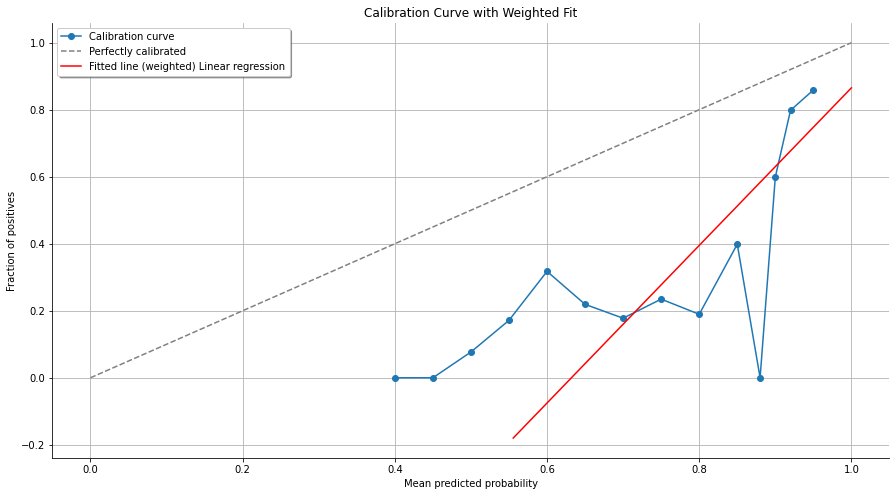
\includegraphics[width=\linewidth]{calibration.png}
	\caption{\textbf{Calibration curve.} Calculated on Gemini model with 6-digit codes as context.}
	\label{fig:column}
\end{figure}


%------------------------------------------------

\section*{Results}


\begin{table}[!htb]
\centering
\resizebox{1.0 \linewidth}{!}{\begin{tabular}{l c c c c c}
\hline
% & &\multicolumn{5}{c}{Number of segmented training images}\\
Model & CA-2 & CA-3 & CA-4 & CA-5 & CA-6 \\ \hline
ChatGPT-4o-mini  & 0.463 & 0.463 & 0.463 & 0.463 & 0.463  \\
ChatGPT-4o-mini (no context)  & 0.463 & 0.463 & 0.463 & 0.463 & 0.463   \\
Gemini-2.0-flash  & 0.51 & 0.463 & 0.463 & 0.463 & 0.463  \\
Gemini-2.0-flash (no context)  & 0.51  & 0.463 & 0.463 & 0.463 & 0.463 \\
\hline
\end{tabular}}
\caption{Performance comparison on test set with manually annotated ground truths. Classification accuracies are divided by the number of correctly classified digits.}
\label{tab:layers}
\end{table}


\subsection*{Hierarchical context}

Due to the hierarchical structure of the codes (first two digits representing a general field, the remaining four representing a specific activity) it is possible to improve most LLM's accuracies by feeding them prompts and contexts hierarchically. That is, first classify the first two digits, where accuracy is generally higher, then progress towards the more detailed labels from there. Results obtained with this approach are shown in Table \ref{tab:context}

\begin{table}[!htb]
\centering
\resizebox{1.0 \linewidth}{!}{\begin{tabular}{l c c c c c}
\hline
% & &\multicolumn{5}{c}{Number of segmented training images}\\
Model & CA-2 & CA-3 & CA-4 & CA-5 & CA-6 \\ \hline
Gemini-2.0-flash  & 0.51 & 0.463 & 0.463 & 0.463 & 0.463  \\
Gemini-2.0-flash (hierarchical)  & 0.51  & 0.463 & 0.463 & 0.463 & 0.463 \\
\hline
\end{tabular}}
\caption{Performance comparison with and without hierarchical context.}
\label{tab:context}
\end{table}


%------------------------------------------------

\section*{Discussion}

 placeholder citation \cite{Demsar2017LinguisticEvolution} 

%------------------------------------------------

\section*{Acknowledgments}

We would like to thank our advisor Erik Štrumbelj for expert guidance and the PredictLeads company for their data and for entrusting us to work on their problem. 


%----------------------------------------------------------------------------------------
%	REFERENCE LIST
%----------------------------------------------------------------------------------------
\bibliographystyle{unsrt}
\bibliography{report}


\end{document}